\chapter{Event Selection}
\label{chap:Selection}

Events are required to contain exactly three \emph{tight} leptons described in \autoref{sec:Leptons}. Furthermore, events are selected with HLT triggers discussed in \autoref{sec:Triggers}. Events with different lepton flavor composites are further categorized into three exclusive channels: eee, $\mmm$, $\emul$. In all three channels, the sum of the electric charges of three selected leptons are required to be 1 or -1. The leading leptons in all selected events are required to be matched with trigger objects via $\mathrm{\Delta} R~<$ 0.2. Within each channel, different regions are defined to further understand signal and background.

$\emul$ is the channel where close to 100\% of the simuated signal events reside. This channel is divided into signal-enriched \acp{SR} and signal-depleted \acp{VR}, which are discussed in \autoref{sec:SR} and \autoref{sec:VR}, respectively. Due to the lack of different flavors, the eee and $\mmm$ channels are signal-depleted by definition. Therefore, events found in these two channels are only used to study background processes, which is discussed in \autoref{sec:VR}. The kinematic reconstruction of heavy particles, such as the top quark, is described in \autoref{sec:Kin}.
%%%%%%%%%%%%%%%%%%%%%%%%%%%%%%%%%%%%%%%%%%%%%%%%%%%%%%%%%%%%%
%%%%%%%%%%%%%%%%%%%%%%%%%%%%%%%%%%%%%%%%%%%%%%%%%%%%%%%%%%%%%
\section{Signal Region}
\label{sec:SR}

The core feature of the signal events is the presence of the \ac{OSDF} lepton pair. It is guaranteed that there is at least one \ac{OSDF} pair in all events residing in $\emul$ channel due to the requirement on electric charges. Leptons that form the \ac{OSDF} pair are referred to as the LFV electron or muon as it is assumed that they originate from the \ac{CLFV} interaction. Based on the event topology of the signal process, further selection criteria are applied to define the \ac{SR}. These selection criteria help achieve an optimal signal to background ratio by removing majority of the background events present in $\emul$ channel. 

At tree-level, signal events are expected to contain one or two jets, which motivates a requirement of at least one jet in \ac{SR}. Furthermore, it is required that there is no more than one b-tagged jet to suppress the contribution from $\ttbar$ events. Another prominent background is Drell-Yan production that features a \ac{OSSF} pair. To suppress Drell-Yan processes in \ac{SR}, events that contain an \ac{OSSF} lepton pair with an invariant mass between 50 GeV and 106 GeV are removed. The lower bound of the this veto is lower than the typical value (e.g. 75 GeV) because the mass range between 50 GeV and 106 GeV has very few signal events and is dominated by \emph{nonprompt} background from photon conversion. Additionally, a modest threshold of 20 GeV is applied to \ac{MET} due to the presence of neutrinos in the signal events.

Distributions of the invariant mass of the \ac{OSDF} pair and the invariant mass of the \ac{OSSF} pair are shown in Figure~\ref{fig:SR}. All backgrounds in Figure~\ref{fig:SR} are estimated using MC simulation even though strategy is to use a data-driven method to estimate the \emph{nonprompt} background. This serves as a preliminary check to understand the components of different backgrounds in \ac{SR}. 

\begin{figure}[tbh!]
 \begin{center}
 \begin{tabular}{cc}
 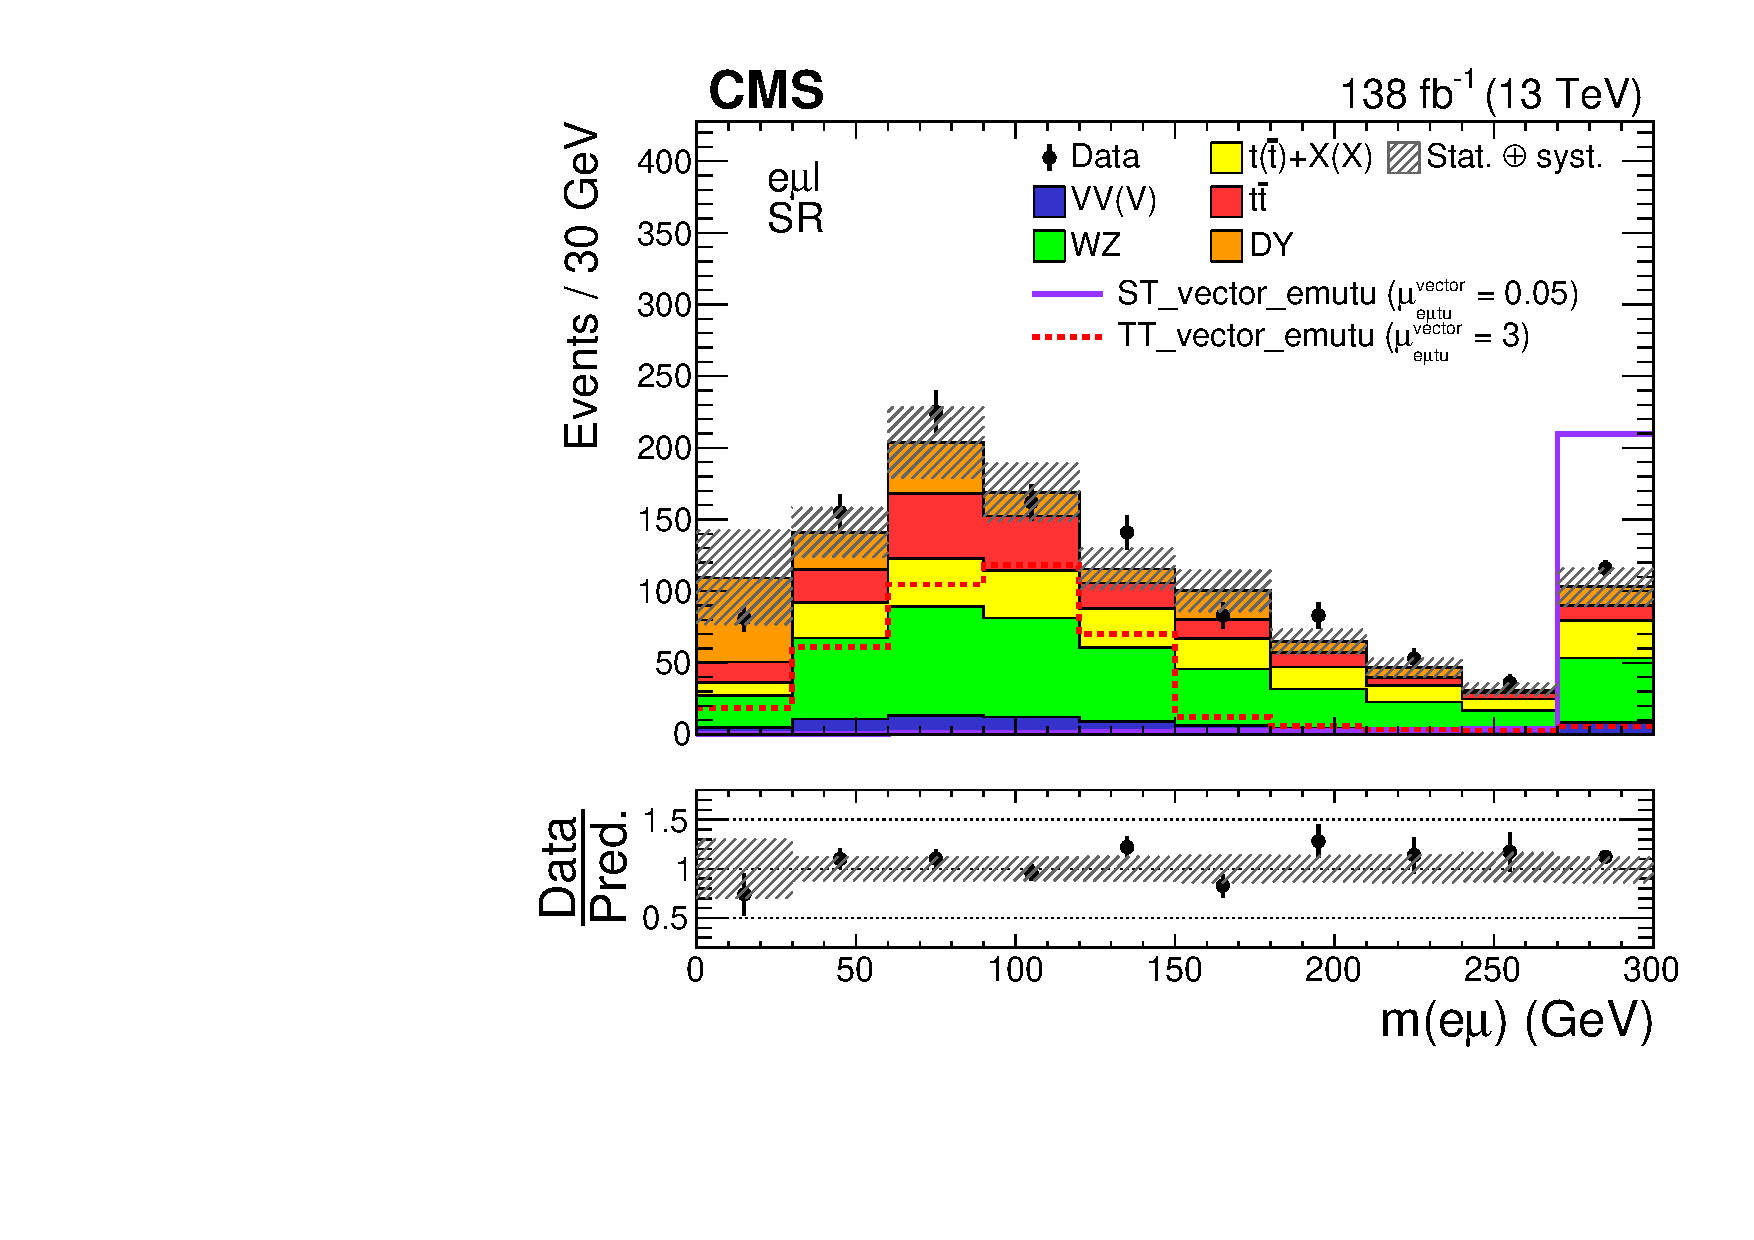
\includegraphics[width=0.45\textwidth]{figures/Part3/Selection/Memu}&
 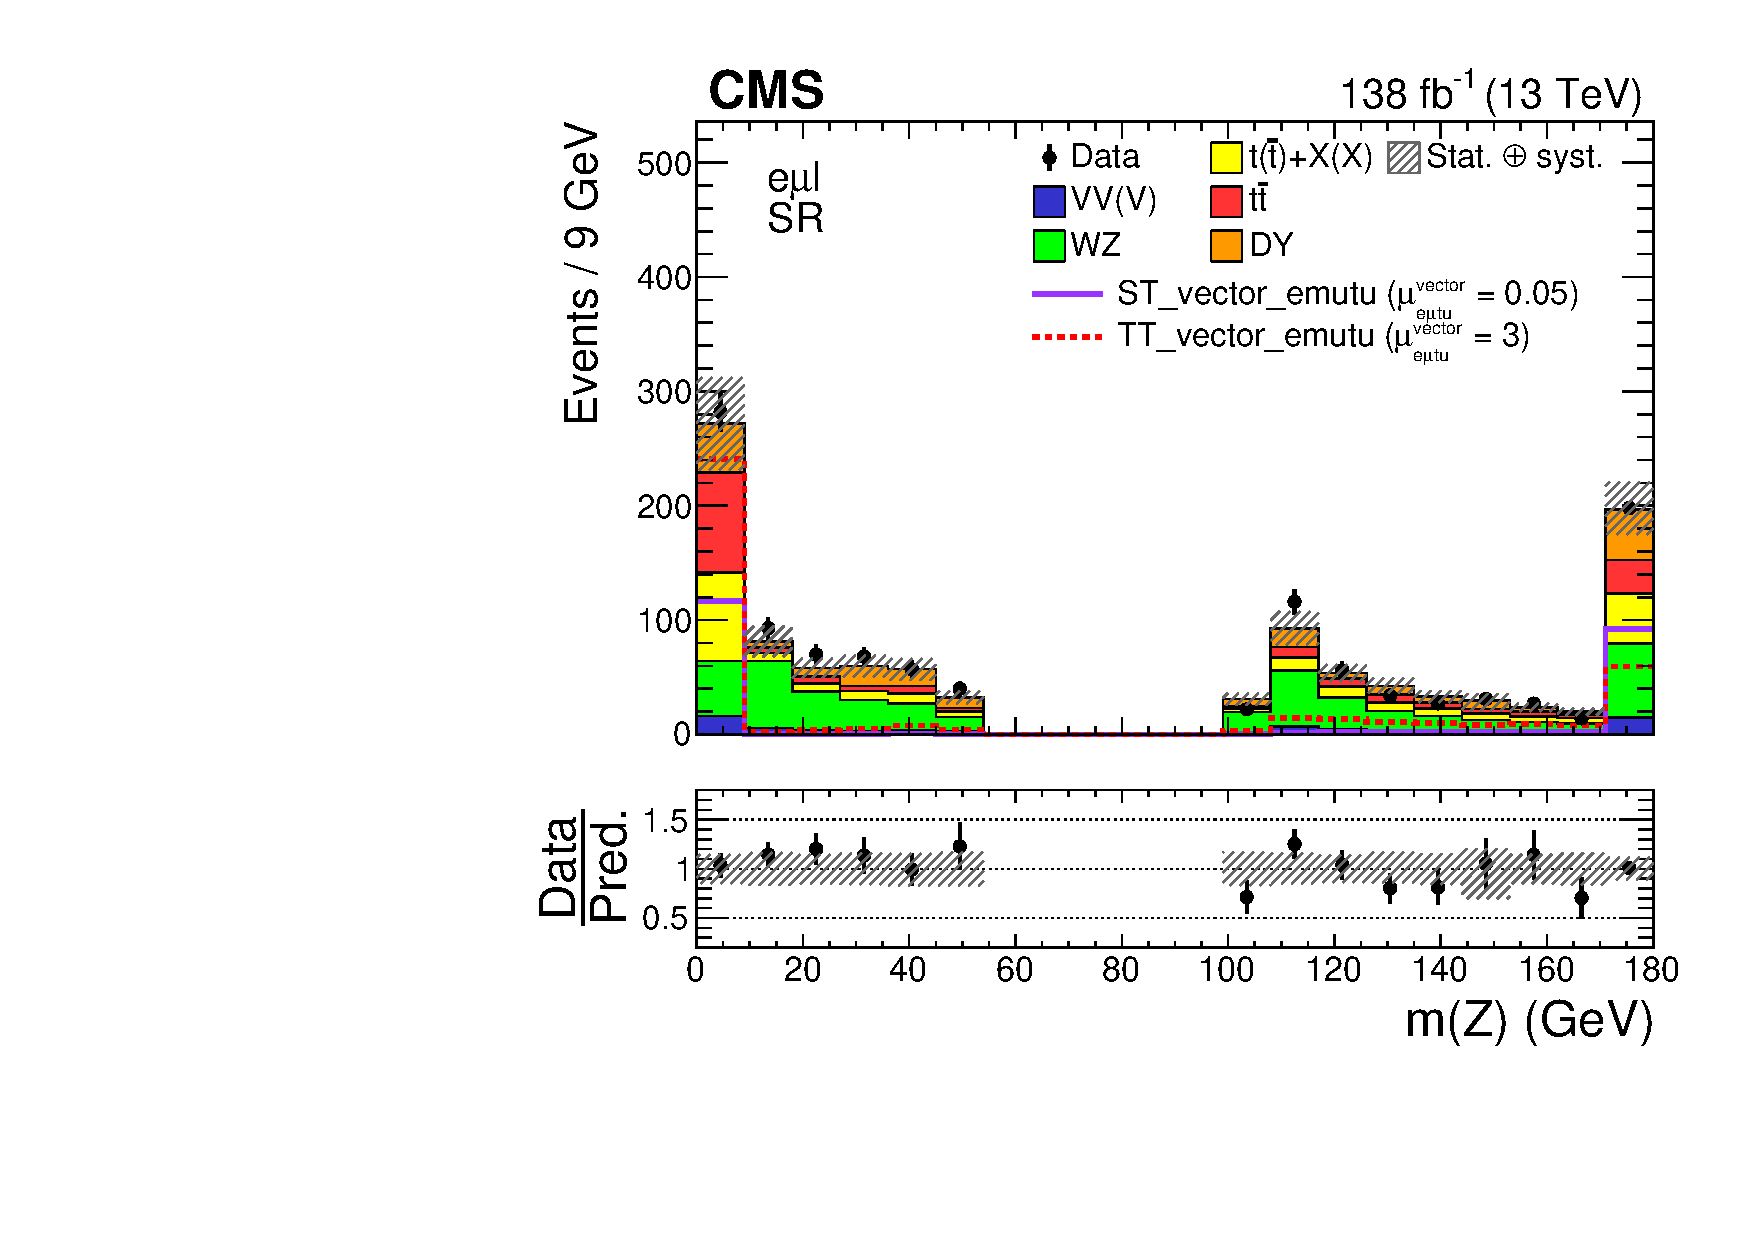
\includegraphics[width=0.45\textwidth]{figures/Part3/Selection/Zmass} \\
 \end{tabular}
 \caption{Distributions of the invariant mass of the \ac{OSDF} pair (left) and the invariant mass of the \ac{OSSF} pair (right) in \ac{SR}. The data are shown as filled points and the \ac{SM} background predictions as histograms. The VV(V) background includes ZZ and triboson production, while the $\ttbar$ + X(X) component includes $\ttbar$W, $\ttbar$Z, $\ttbar$H, tZq, and smaller backgrounds containing one or two top quarks plus a boson or quark. All backgrounds are estimated using \ac{MC} simulation. The hatched bands indicate statistical and systematic uncertainties for the \ac{SM} background predictions. The last bin of both histograms includes the overflow events.}
 \label{fig:SR}
 \end{center}
\end{figure}

Using the invariant mass of the \ac{OSDF} pair, \ac{SR} is further divided into two subsets to create top production and decay enriched regions:

\begin{itemize}
\item SR1, $\textsf{m}_{\textsf{e}\upmu}~<$ 150 GeV: top decay enriched.
\item SR2, $\textsf{m}_{\textsf{e}\upmu}~>$ 150 GeV: top production enriched.
\end{itemize}
%%%%%%%%%%%%%%%%%%%%%%%%%%%%%%%%%%%%%%%%%%%%%%%%%%%%%%%%%%%%%
%%%%%%%%%%%%%%%%%%%%%%%%%%%%%%%%%%%%%%%%%%%%%%%%%%%%%%%%%%%%%
\section{Validation Region}
\label{sec:VR}

\begin{figure}[tbh!]
 \begin{center}
 \begin{tabular}{c}
 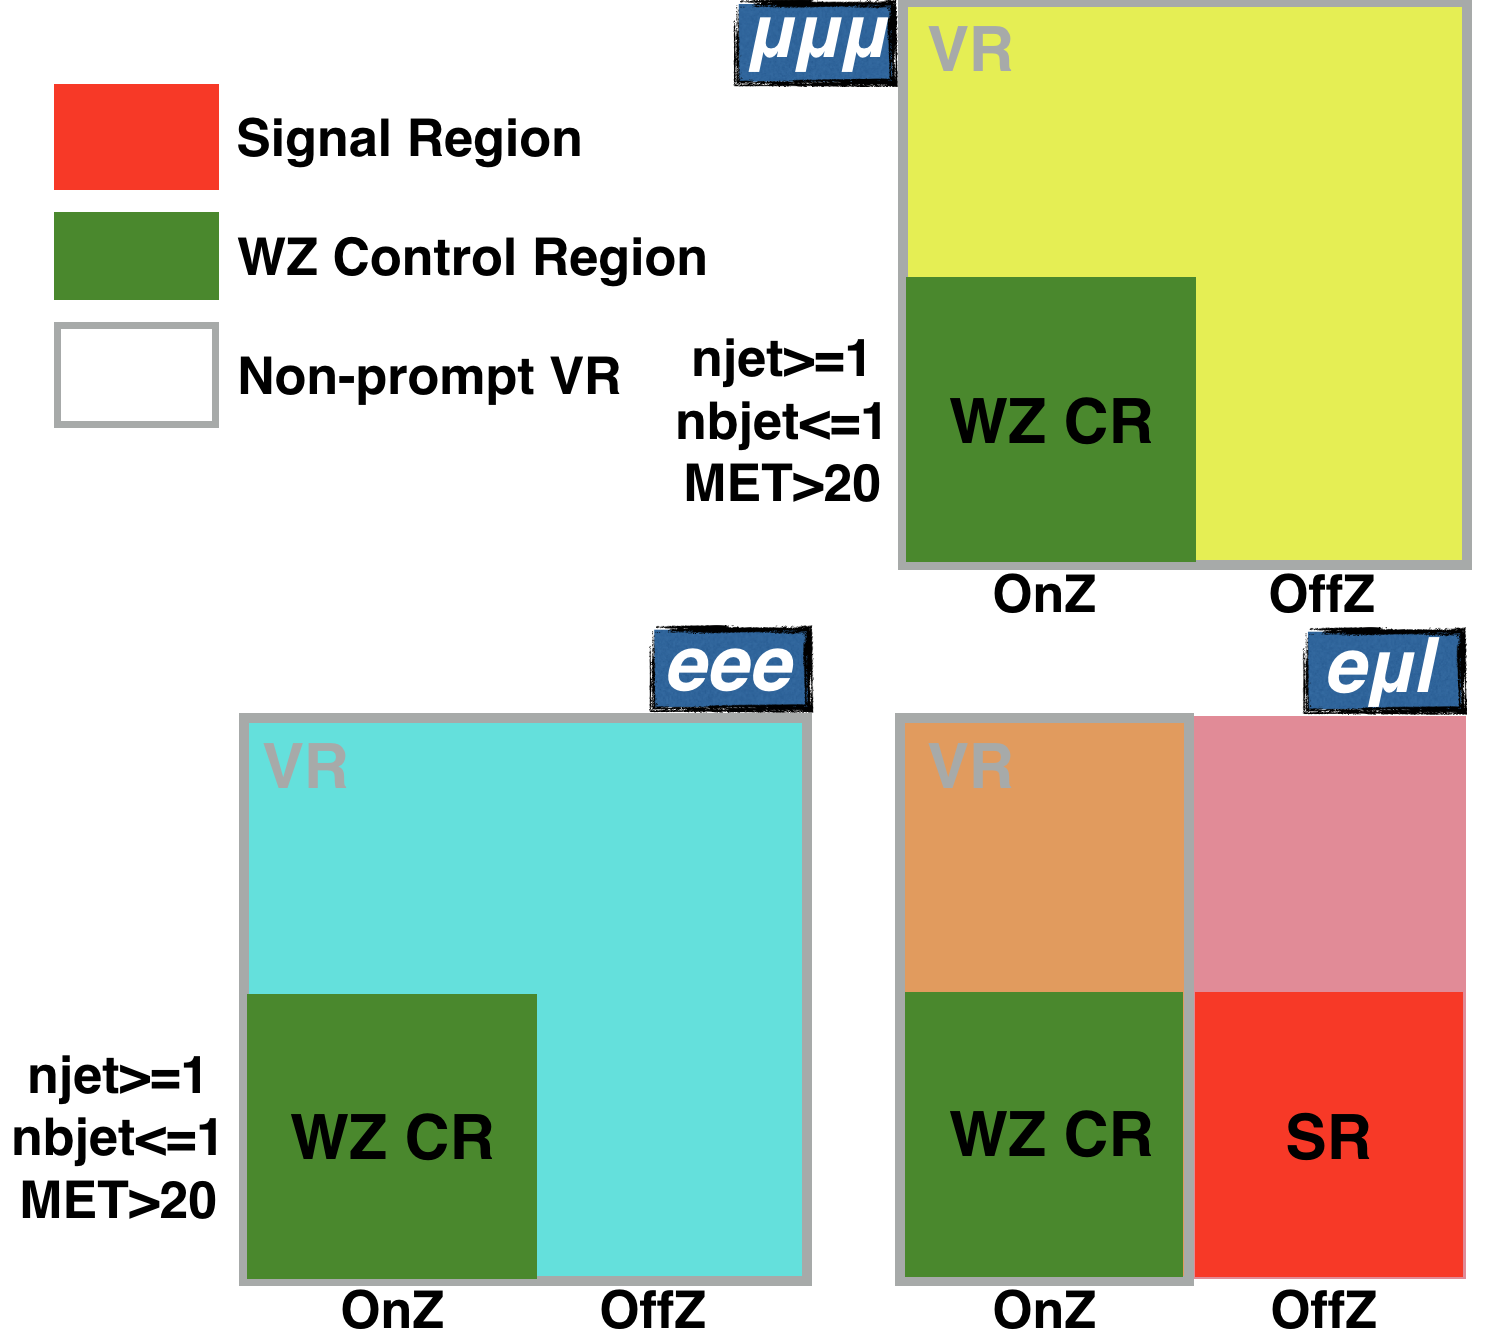
\includegraphics[width=0.8\textwidth]{figures/Part3/Selection/Event}
 \end{tabular}
 \caption{Illustration of selection criteria used to define different regions. ``OnZ'' means the presence of at least one \ac{OSDF} pair with an invariant mass between 50 GeV and 106 GeV. Events are labelled as ``OffZ'' when they fail ``OnZ'' criteria.}
 \label{fig:Event}
 \end{center}
\end{figure}

There are two types of signal-depleted \ac{VR} defined across three channels: \emph{nonprompt} \ac{VR} and WZ \ac{VR}. The purpose of these two types of \ac{VR} is only limited to the validation of the background modelling as neither of them enter the final fit. It is expected that the \emph{nonprompt} \ac{VR} has a significant fraction of \emph{nonprompt} background while WZ production is responsible for most of the backgrounds in the WZ \ac{VR}. Distributions of leading lepton $\pt$ and leading lepton $\eta$ in WZ control region can be found in Figure~\ref{fig:WZ_eee}-\ref{fig:WZ_mumumu}. The \emph{nonprompt} \ac{VR} are further discussed in \autoref{chap:Nonprompt}.

Selection criteria used to define different regions are illustrated in Figure~\ref{fig:Event} and is summarized in Table~\ref{tab:region}.

\begin{figure}[tbh!]
 \begin{center}
 \begin{tabular}{cc}
 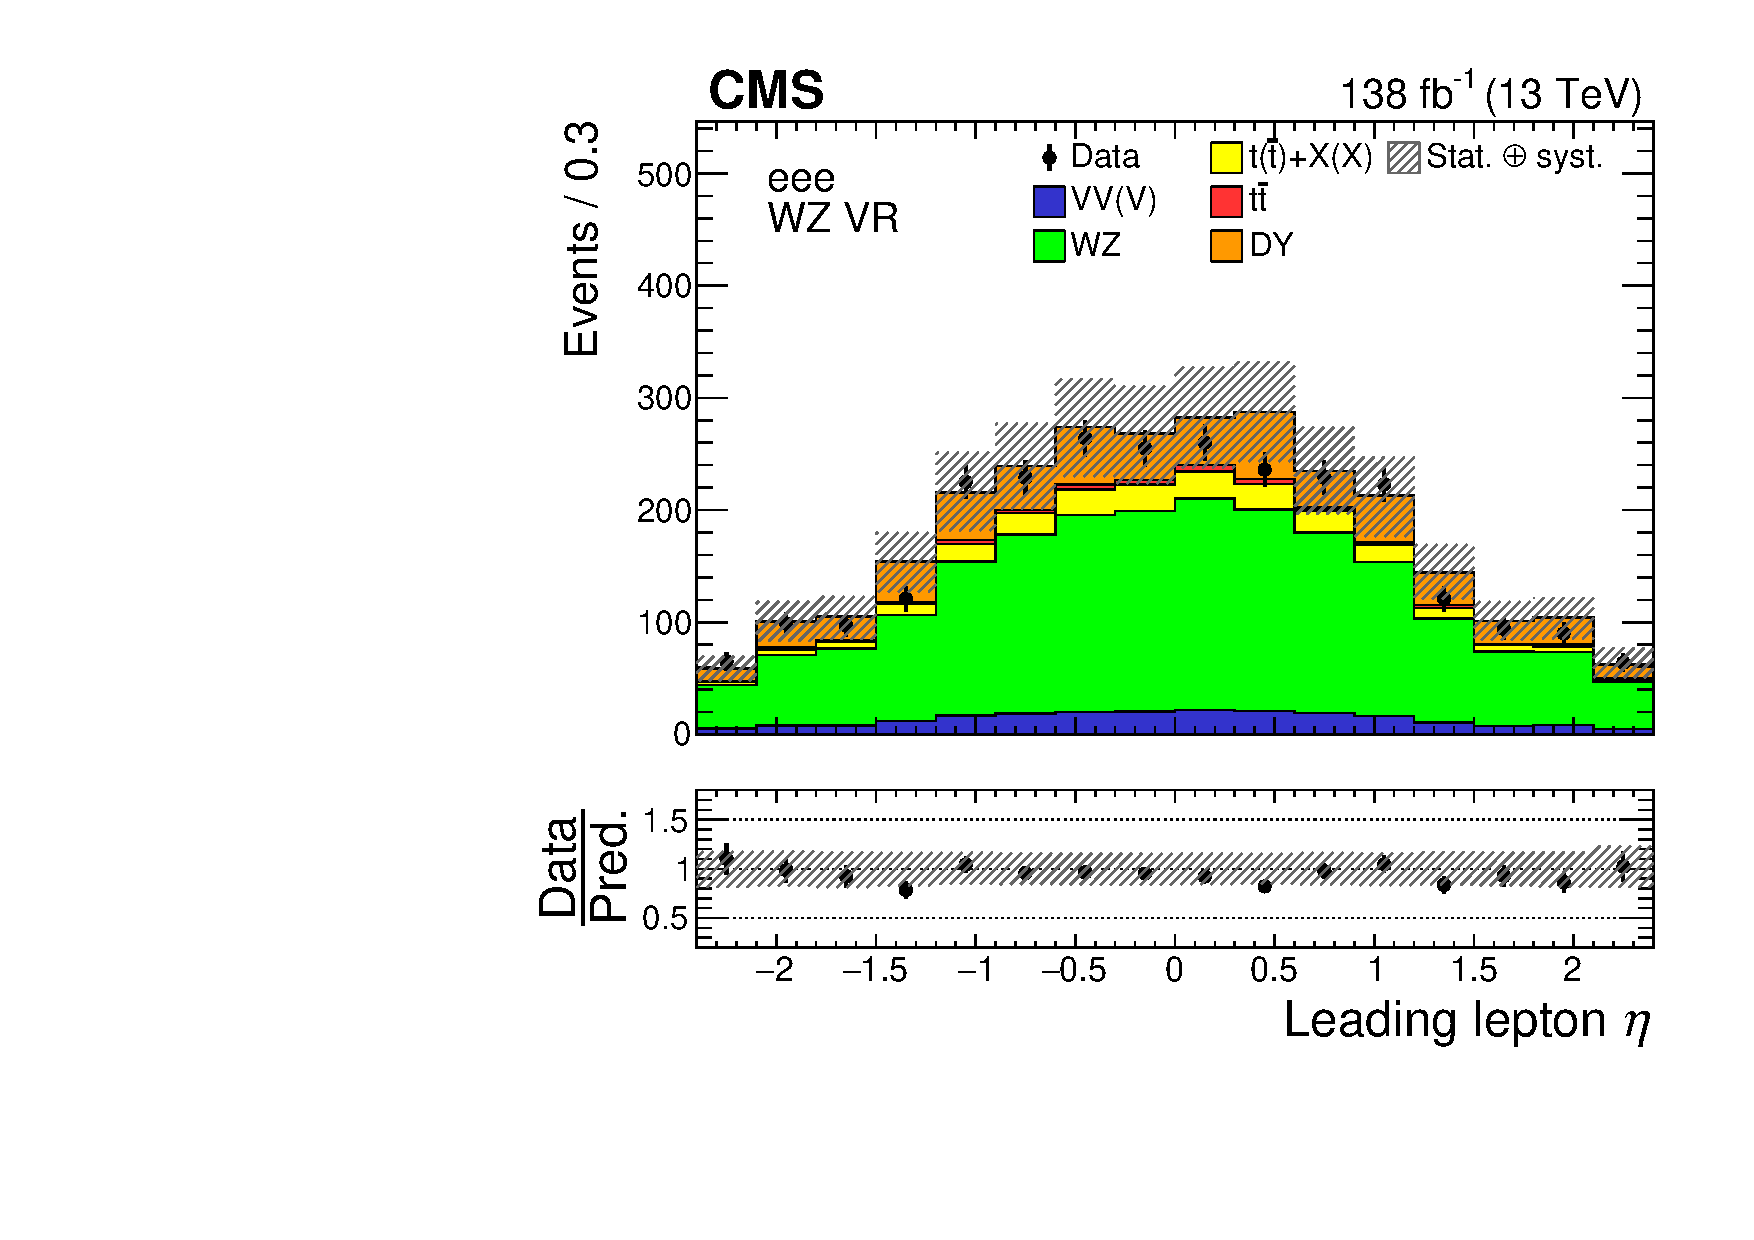
\includegraphics[width=0.45\textwidth]{figures/Part3/Selection/WZ/eee/lep1Eta}&
 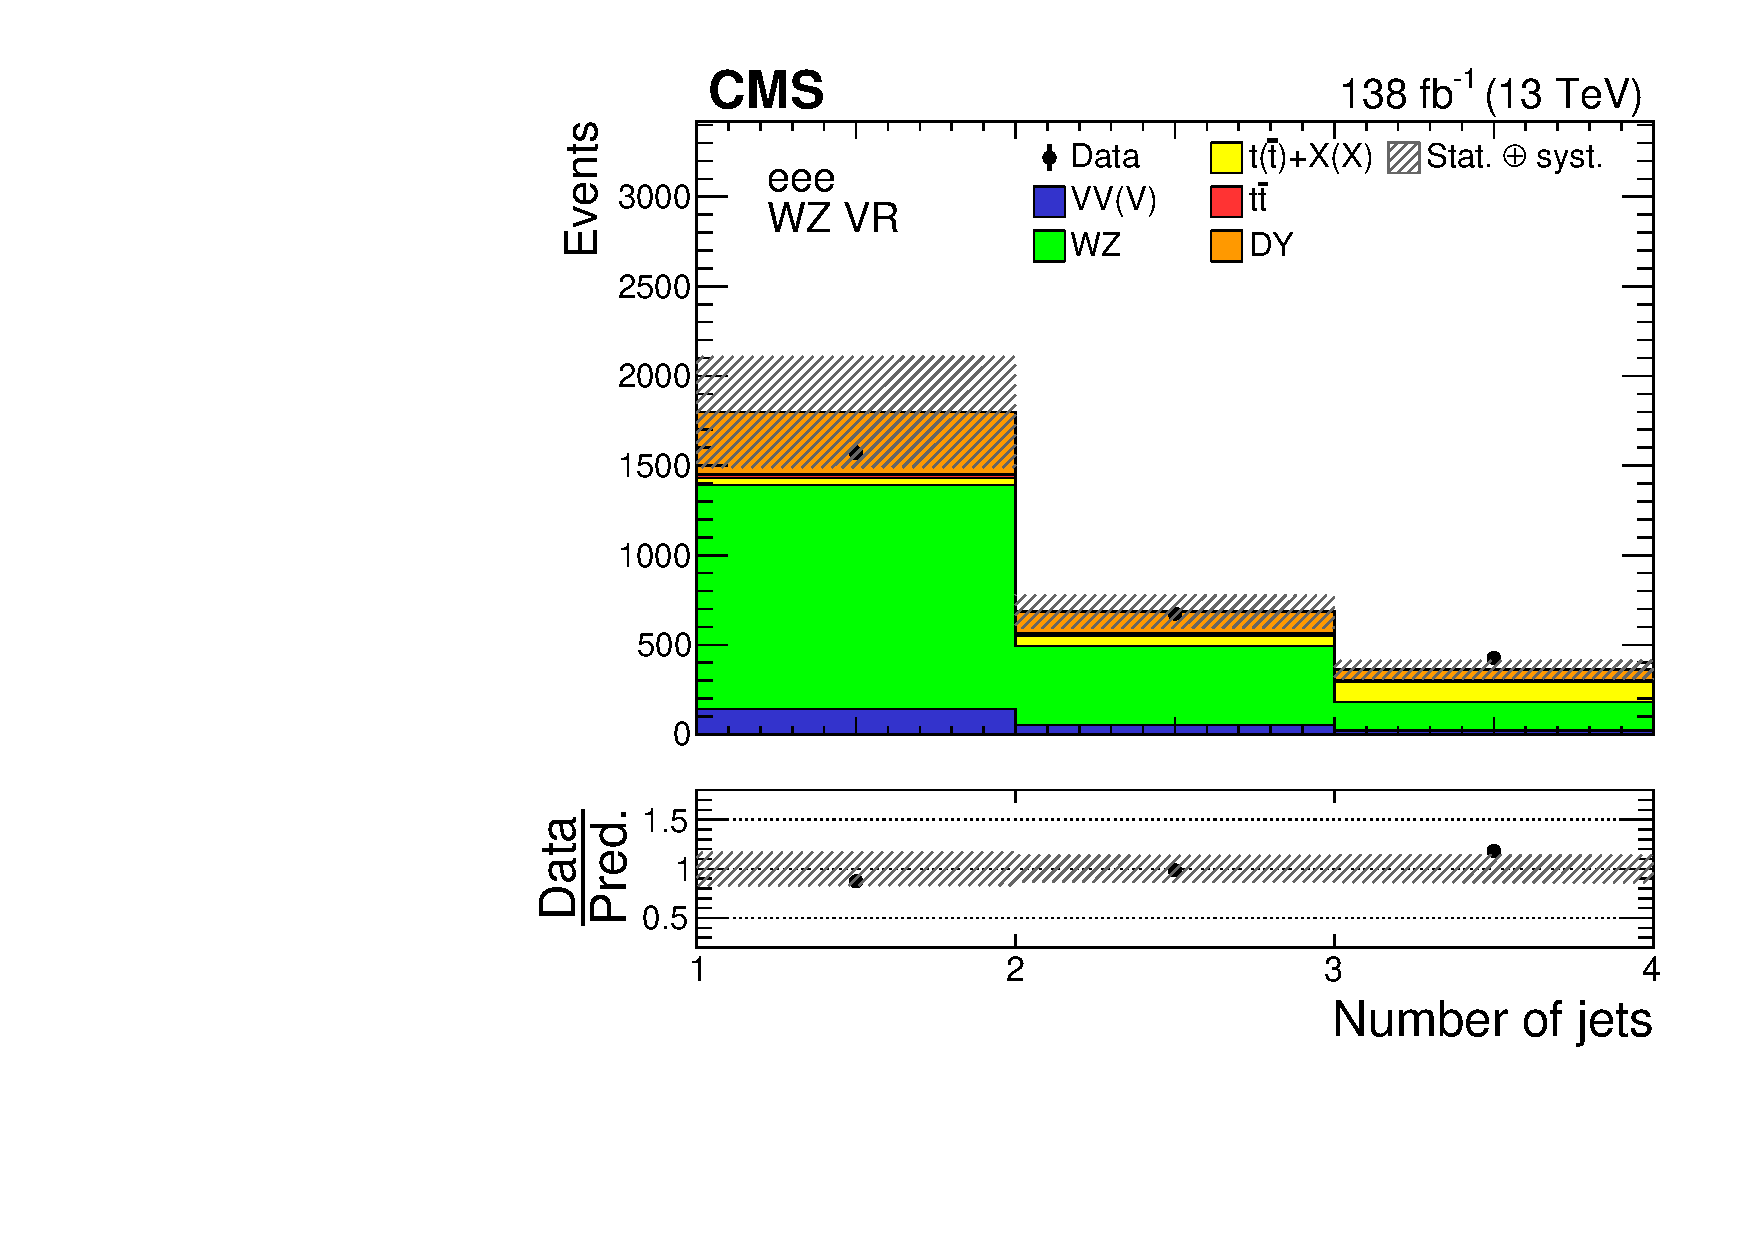
\includegraphics[width=0.45\textwidth]{figures/Part3/Selection/WZ/eee/njet} \\
 \end{tabular}
 \caption{Distributions of different kinematic variables estimated in WZ control region (full run II). Backgrounds are estimated using MC only. From left to right: leading lepton $\eta$, jet multiplicity.}
 \label{fig:WZ_eee}
 \end{center}
\end{figure}

\begin{figure}[tbh!]
 \begin{center}
 \begin{tabular}{cc}
 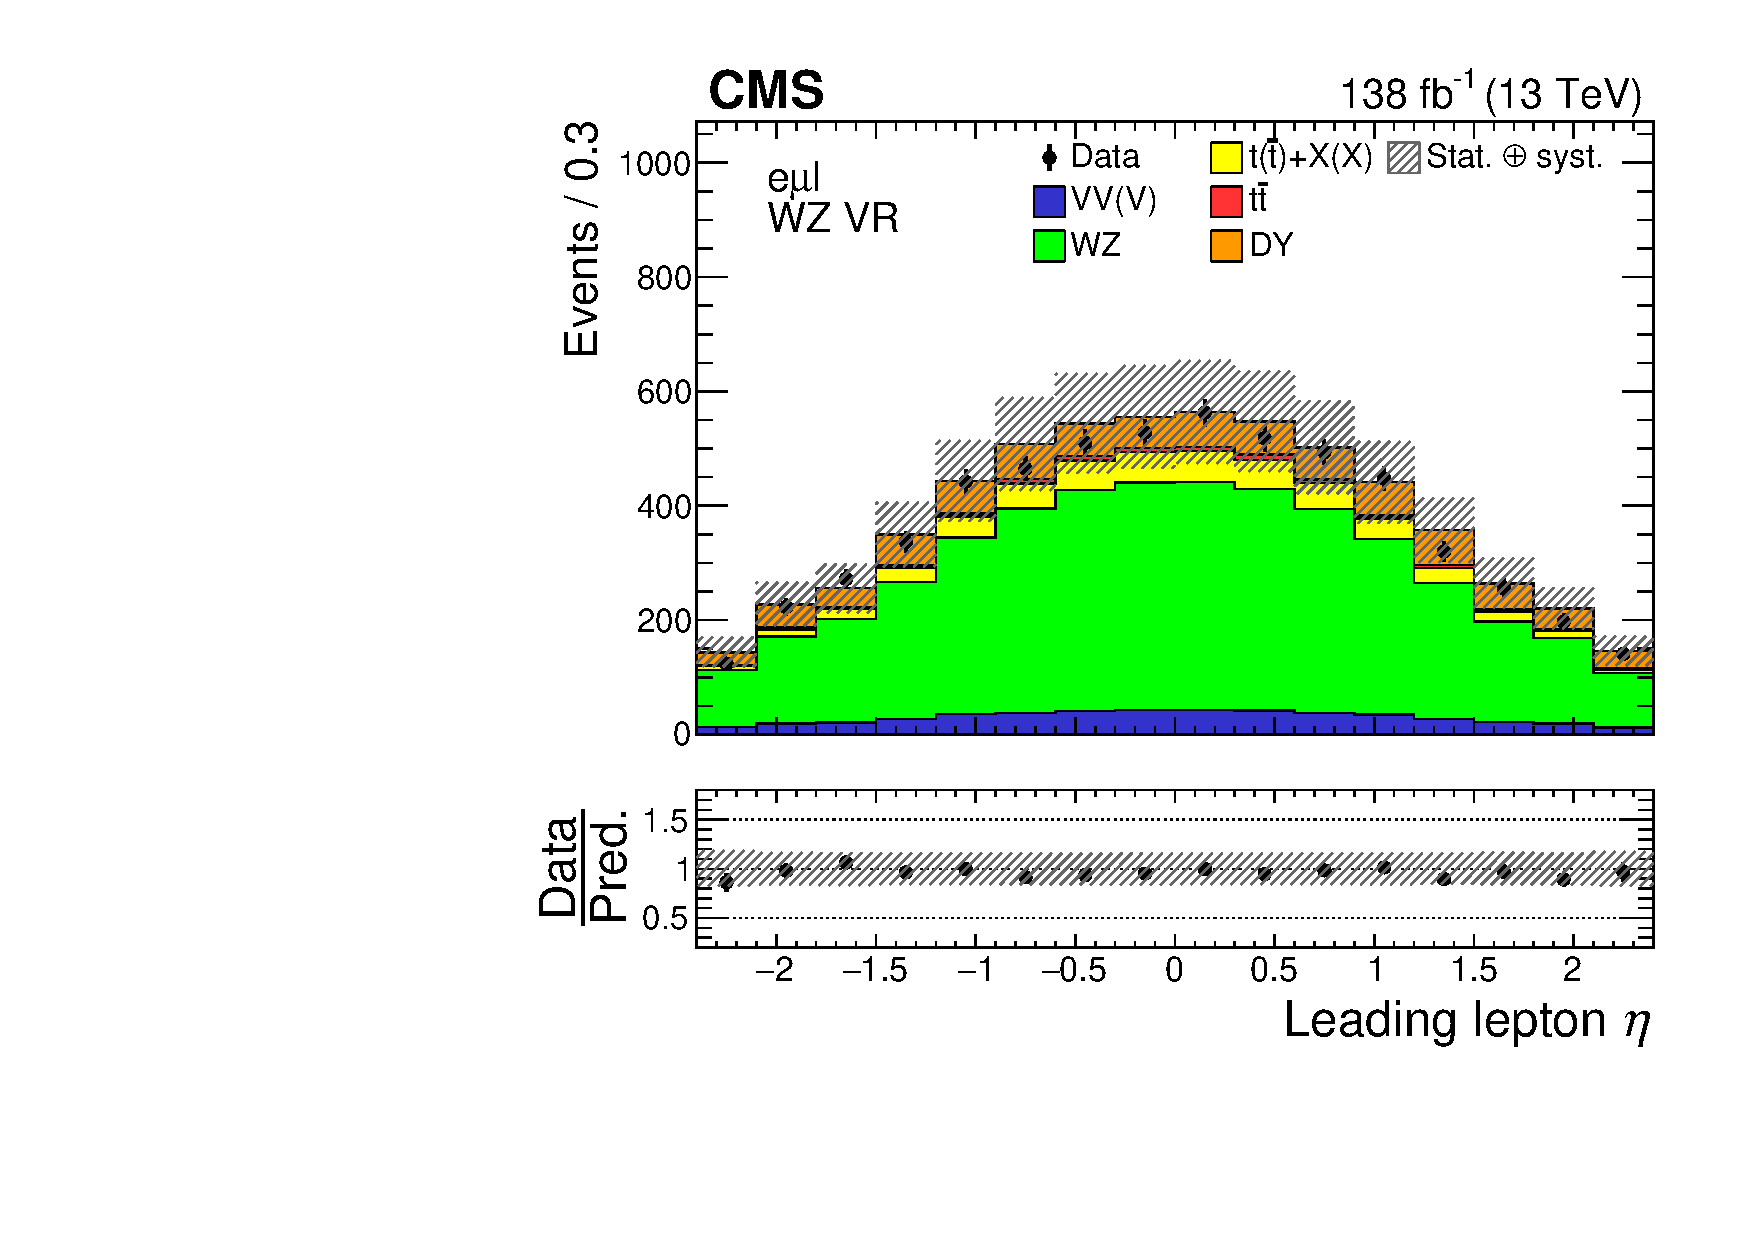
\includegraphics[width=0.45\textwidth]{figures/Part3/Selection/WZ/emul/lep1Eta}&
 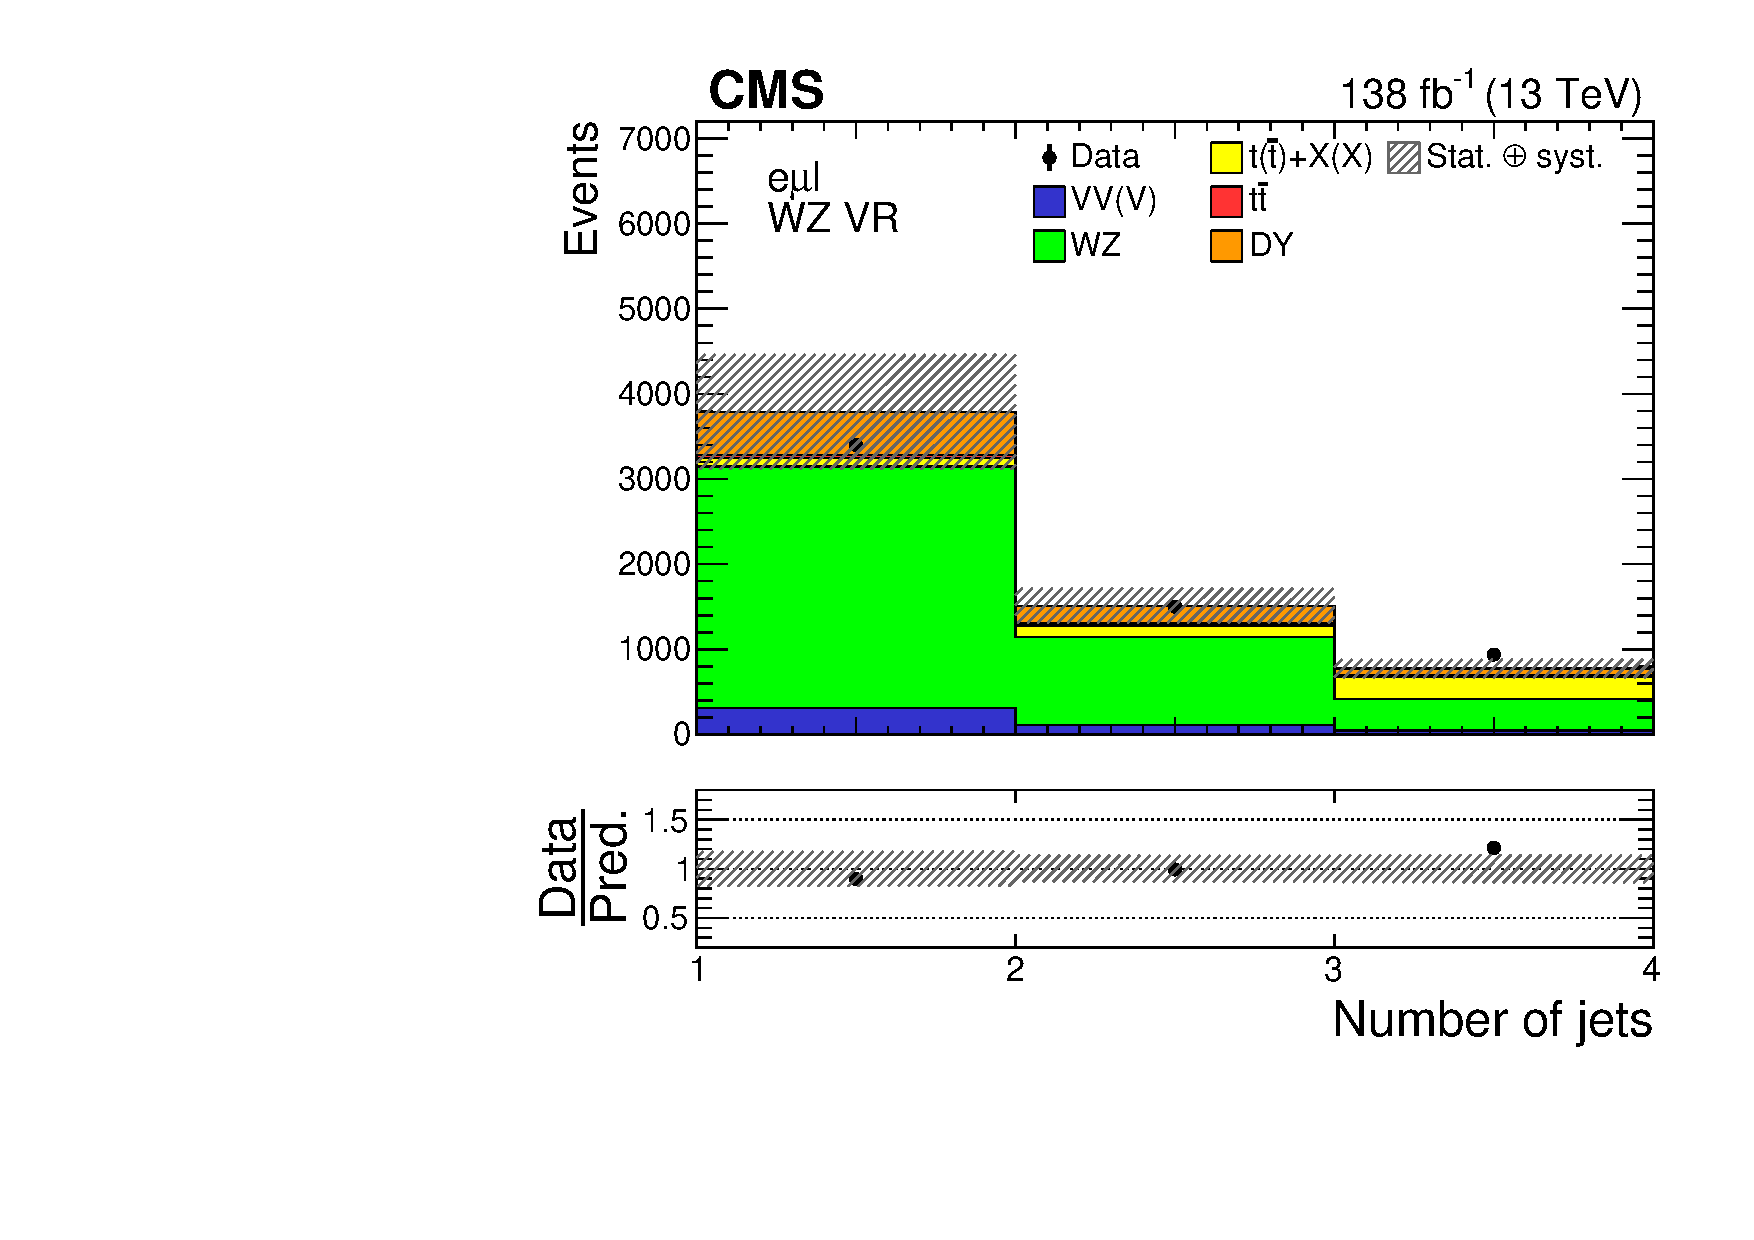
\includegraphics[width=0.45\textwidth]{figures/Part3/Selection/WZ/emul/njet} \\
 \end{tabular}
 \caption{Distributions of different kinematic variables estimated in WZ control region (full run II). Backgrounds are estimated using MC only. From left to right: leading lepton $\eta$, jet multiplicity.}
 \label{fig:WZ_emul}
 \end{center}
\end{figure}

\begin{figure}[tbh!]
 \begin{center}
 \begin{tabular}{cc}
 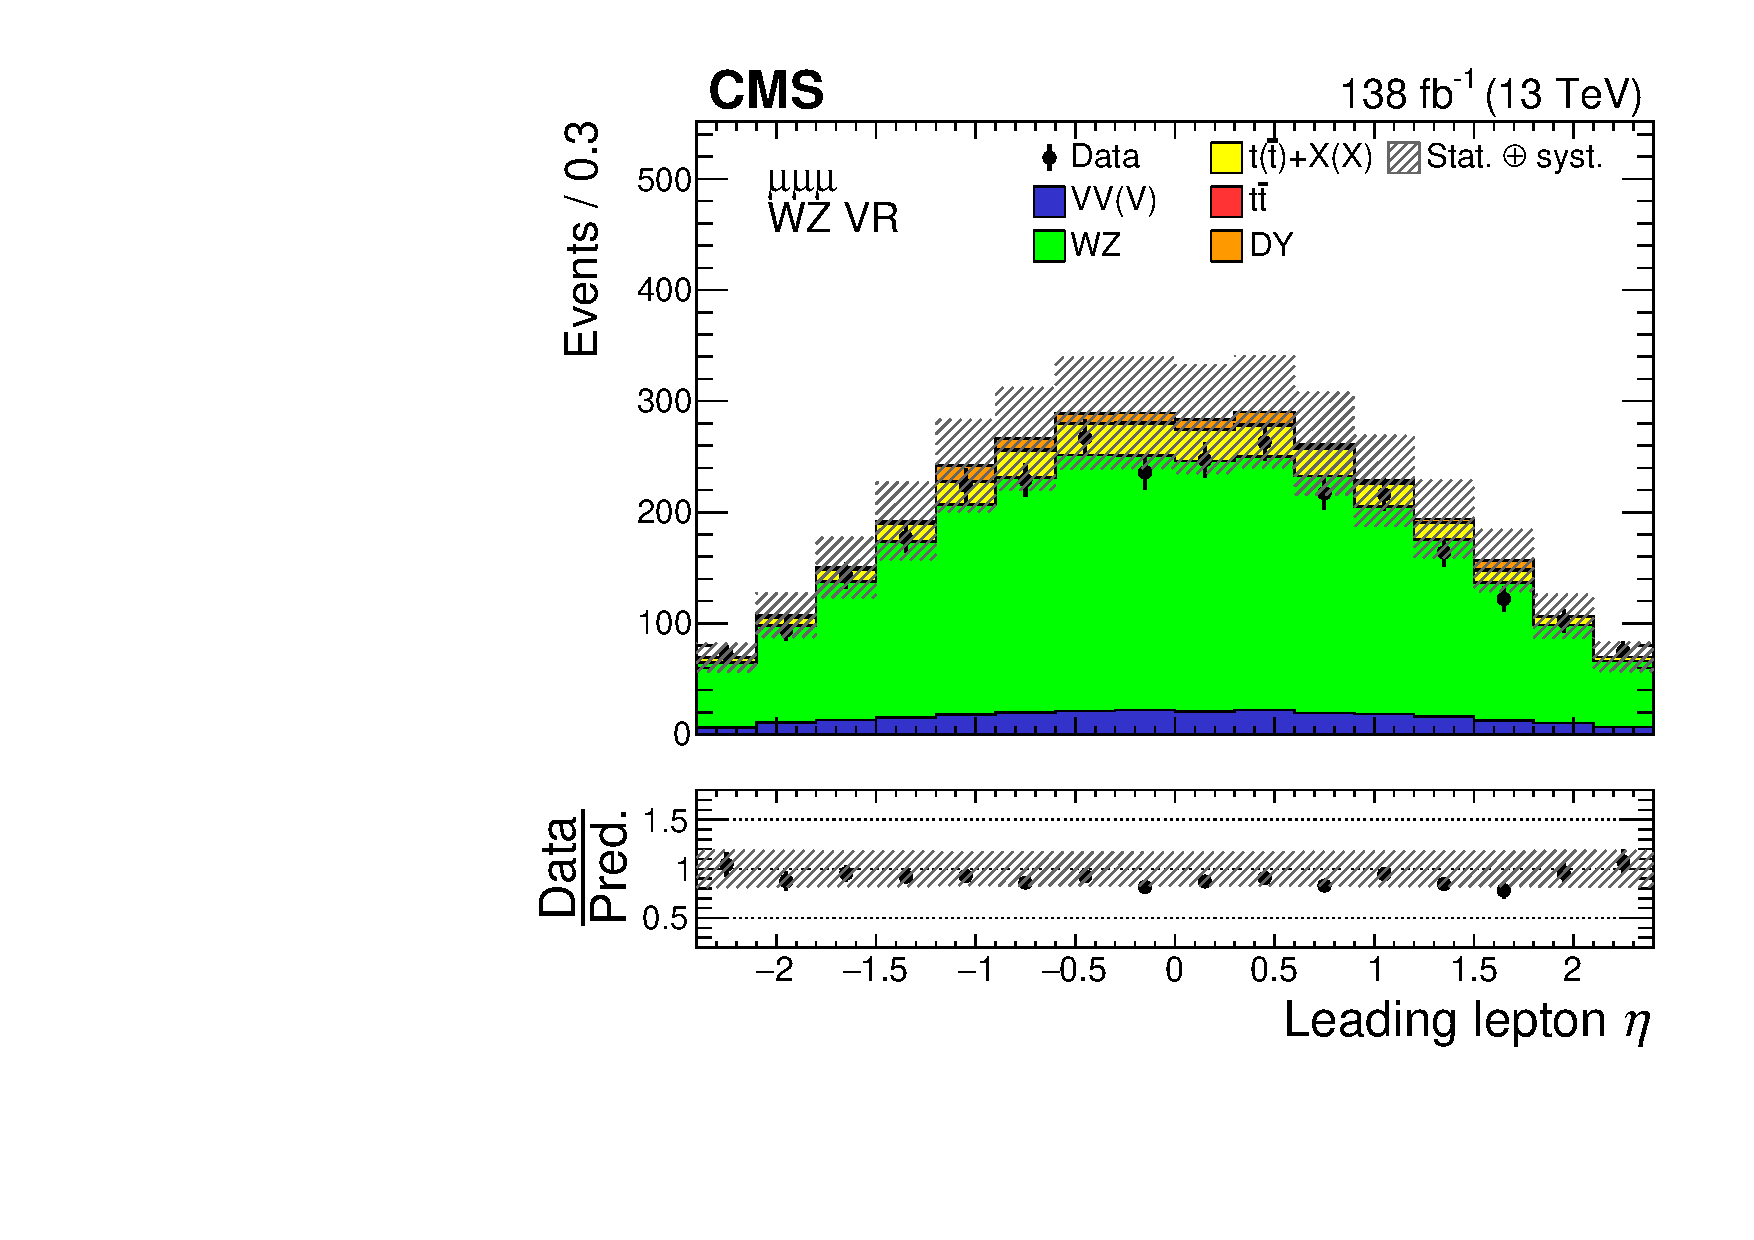
\includegraphics[width=0.45\textwidth]{figures/Part3/Selection/WZ/mumumu/lep1Eta}&
 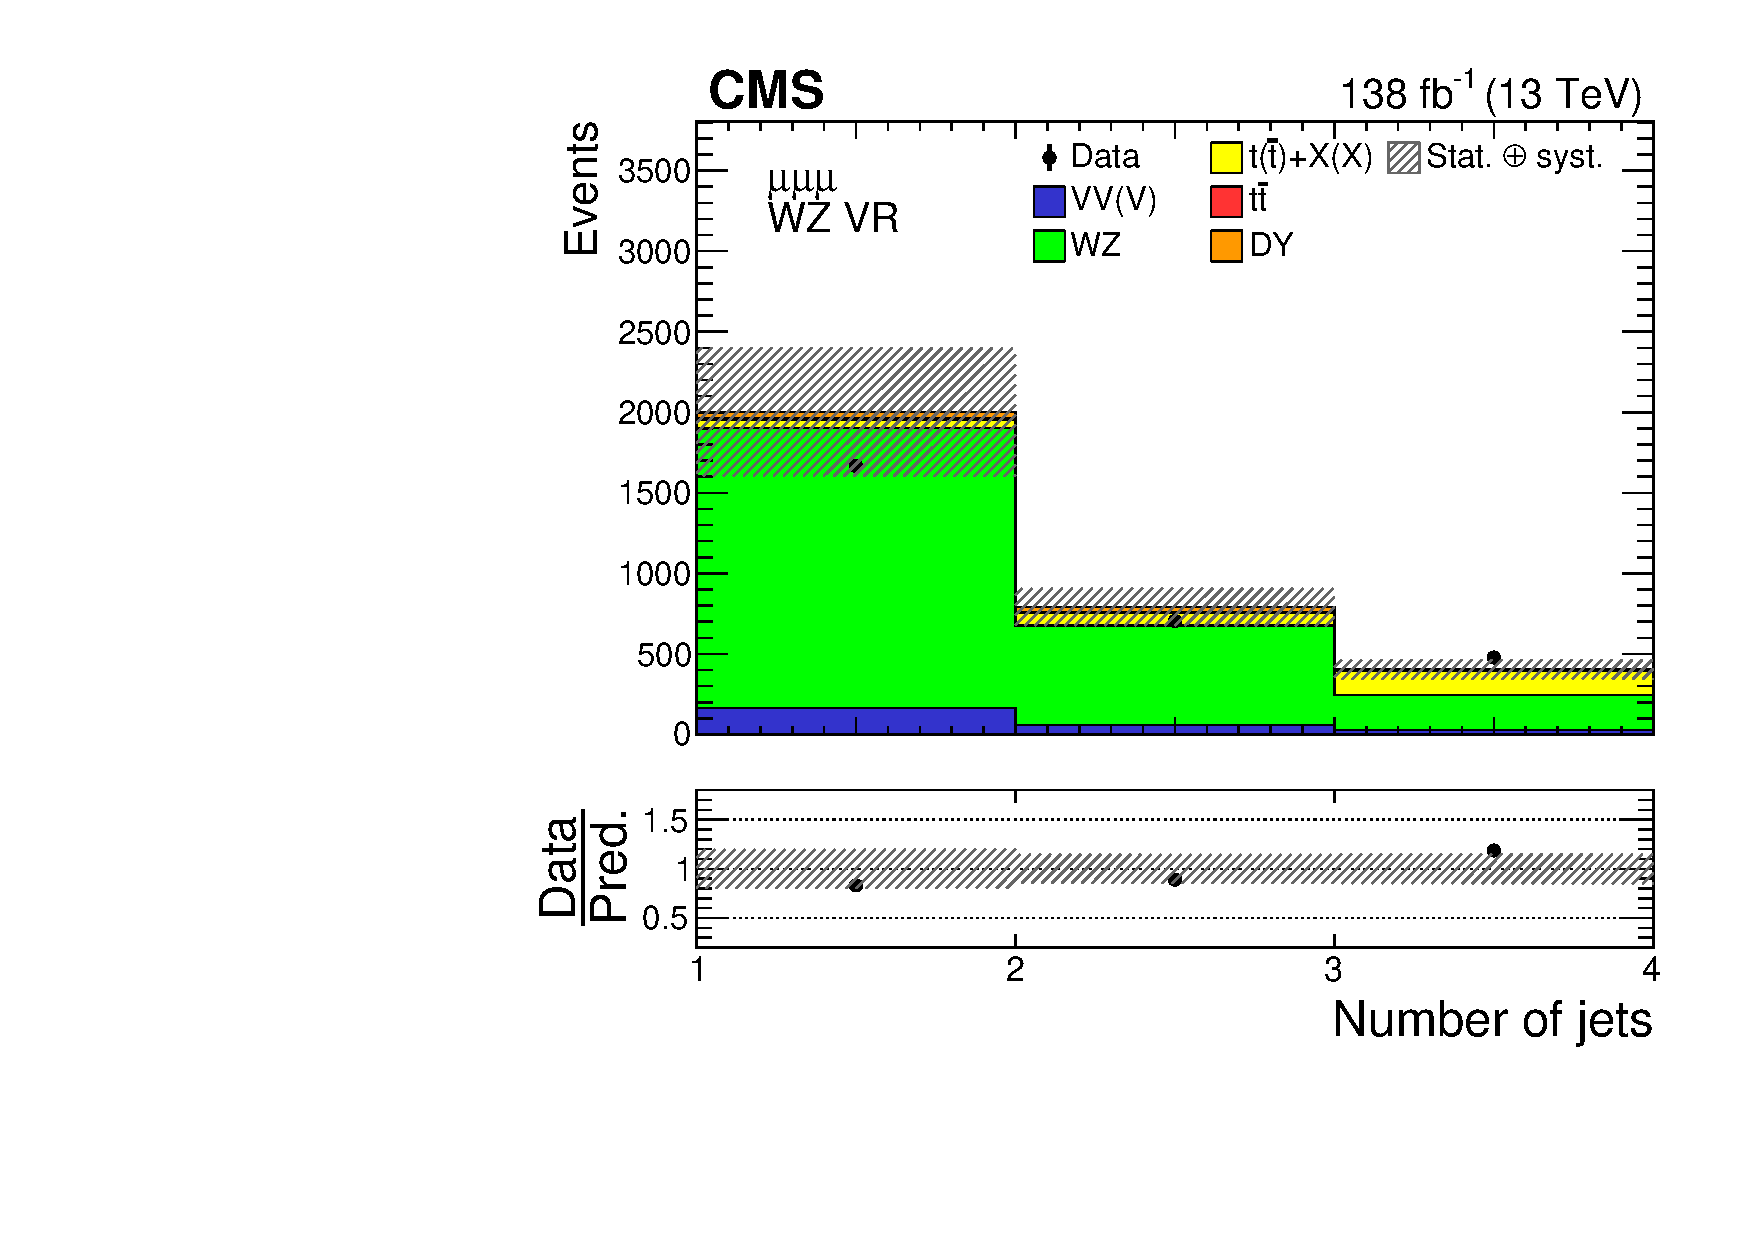
\includegraphics[width=0.45\textwidth]{figures/Part3/Selection/WZ/mumumu/njet} \\
 \end{tabular}
 \caption{Distributions of different kinematic variables estimated in WZ control region (full run II). Backgrounds are estimated using MC only. From left to right: leading lepton $\eta$, jet multiplicity.}
 \label{fig:WZ_mumumu}
 \end{center}
\end{figure}

\begin{table}[th]
\sffamily
\centering
\begin{tabular}{cccccccc}
\toprule
Channel         &Region & OnZ & OffZ & MET $>$ 20 GeV &njet$>=$1 &nbjet$<=$1\\ \midrule
\multirow{2}{*}{eee}     & VR  & -       & -       & -       & -     & -   \\  
            & WZ VR & \checkmark   & -       & \checkmark   & \checkmark & \checkmark\\ \midrule
\multirow{3}{*}{e$\upmu\ell$}   & SR   & -       & \checkmark   & \checkmark   & \checkmark & \checkmark \\
            & Nonprompt VR   & \checkmark   & -       & -       & -     & -     \\
            & WZ VR  & \checkmark   & -       & \checkmark   & \checkmark & \checkmark \\ \midrule
\multirow{2}{*}{$\upmu\upmu\upmu$} & Nonprompt VR    & -       & -       & -       & -     & -     \\  
            & WZ VR  & -       & \checkmark   & \checkmark & \checkmark & \checkmark  \\ \bottomrule  
\end{tabular}
\caption{Summary of the selection criteria used to define different event regions. ``OnZ'' means the presence of at least one \ac{OSDF} pair with an invariant mass between 50 GeV and 106 GeV. Events are labelled as ``OffZ'' when they fail ``OnZ'' criteria.}
\label{tab:region}
\end{table}
%%%%%%%%%%%%%%%%%%%%%%%%%%%%%%%%%%%%%%%%%%%%%%%%%%%%%%%%%%%%%
%%%%%%%%%%%%%%%%%%%%%%%%%%%%%%%%%%%%%%%%%%%%%%%%%%%%%%%%%%%%%
\section{Kinematic Reconstruction}
\label{sec:Kin}

As mentioned, the \ac{OSDF} lepton pair in the $\emul$ channel is assumed to be the product of the \ac{CLFV} interaction, while the third lepton, referred to as the standalone lepton, is assumed to originate from the leptonically decaying top quark. To distinguish this top quark (t$\rightarrow\ell\nu$b) with the top quark that decays via the \ac{CLFV} interaction. The former is referred to as the \ac{SM} top quark while the latter is referred to as the LFV top quark. Jet with the highest b-tagging score, regardless of whether or not it crosses the medium working point threshold, is assumed to originate from bottom quark decay. Therefore, it is combined with \ac{MET} and the standalone lepton to build the \ac{SM} top quark. 

\begin{itemize}
\item We take the x and y component of MET as measurements of neutrino $p_x$ and $p_y$. 
\item The z component of neutrino momentum is calculated by imposing the constraint that the invariant mass of the combined object (bachelor lepton+neutrino) must be equal to W boson mass.
\item If there is no real solution, we take the real part of the complex solution.
\item If there is more than one real solution, we chose the solution that is the closest to the $p_z$ of the bachelor lepton.
\end{itemize}

In events where there is more than one candidate of bachelor lepton, the lepton that gives a top mass that is the closest to the the SM top-quark mass is chosen as the bachelor lepton.

Once the bachelor lepton has been determined, the OSOF pair is combined with jets One-By-One to reconstruct LFV top candidates. Jet with the highest b-tagging score is excluded from this reconstruction since it is assumed to be from the decay of the SM top-quark. Out of all the LFV top candidates, the candidate that gives a top mass that is the closest to the the SM top-quark mass is chosen.

Kinematic reconstruction of heavy objects like top-quark is carried out using selected leptons, jets, and MET.
\begin{itemize}
\item \textbf{Z boson candidate}
\begin{itemize}
\item Z boson candidate is reconstructed by combining two Opposite-Sign-Same-Flavor leptons 
\item Whenever possible, Z candidate with an invariant mass that is closest to Z boson mass is chosen
\end{itemize}
\item \textbf{Standard model top-quark candidate }
\begin{itemize}
\item Standard model top-quark candidate is reconstructed by combining a jet, a lepton, and MET
\item Jet with the highest b-tagging score is always chosen
\item In $e\mu l$ channel, flavor-violating leptons are excluded from reconstruction 
\begin{itemize}
\item Whenever more than one lepton is available due to possible combinatorics of flavor-violating $e\mu$ pair, lepton that forms a top-quark candidate with an invariant mass that is closest to the top-quark mass is chosen 
\end{itemize}
\item In $eee$/$\mu\mu\mu$ channel, leptons that form Z candidate are excluded 
\item Lepton is combined with MET to reconstruct W candidate 
\begin{itemize}
\item Transverse component of the neutrino momentum is taken from MET
\item Neutrino $p_z$ is obtained by W mass constrain set on the lepton-neutrino system 
\end{itemize}
\end{itemize}
\item \textbf{Flavor-violating top-quark candidate }
\begin{itemize}
\item Flavor-violating top-quark candidate is reconstructed by combining a jet and an Opposite-Sign $e\mu$ lepton pair
\item Jet with the highest b-tagging score is excluded from reconstruction unless it fails b-tagging 
\item Whenever possible, the jet that forms a flavor-violating top-quark candidate with an invariant mass that is the closest to the top-quark mass is chosen
\item Lepton that forms the standard model top-quark candidate is excluded 
\end{itemize}
\item \textbf{The first b-jet+lepton system }
\begin{itemize}
\item Jet with the highest b-tagging score is always chosen 
\item All three leptons can form this system with the chosen jet 
\begin{itemize}
\item Lepton that forms a jet-lepton system with the lowest invariant mass is chosen 
\end{itemize}
\end{itemize}
\item \textbf{The second b-jet+lepton system}
\begin{itemize}
\item Jet with the highest b-tagging score is excluded unless it passes b-tagging 
\item Whenever possible (after the previous step), jet with the highest b-tagging score is chosen 
\item Lepton that forms the first jet-lepton system is excluded 
\item Leptons that have the same sign as the lepton that forms the first jet-lepton system is excluded 
\item Whenever possible, lepton that forms a jet-lepton system with the lowest invariant mass is chosen 
\end{itemize}
\end{itemize}